\section{Kommunikation}
\label{sec:com}

Dieses Kapitel geht im näheren auf die Kommunikation zwischen dem Sensor und dem Evaluation System ein. 


\subsection{Anforderungen}

Die Kommunikation zwischen dem Sensor und dem Evaluation System ist ein wesentlicher Bestandteil des gesamten Projektes. Im nächsten Abschnitt wird näher auf die Anforderungen dieser eingegangen.

\begin{description}
  \item[Mobilität:]
  Das System soll so ausgelegt sein, dass die Eltern das Kind auch einfach aus dem Bett heben können ohne vorher Kabelverbindungen trennen zu müssen oder das Gefahr besteht das System dabei zu beschädigen. Daher soll eine kabellose Verbindung verwendet werden.
  
  \item[Einfachheit:]
  Für die Entwicklung des Prototyps sollte die Kommunikation nicht zu Komplex gestalltet werden um die vorhandenen personellen Ressourcen nicht zu übersteigen. 
  
  \item[Energie sparend:]
  Da der Sensor langfristig über einen Akku betrieben werden soll, ist es nötig auf eine Energie sparende Technology zu setzen, damit der Akku nicht jeden Tag geladen werden muss.
  
  \item[Reichweite:]
  Die maximale Reichweite muss ca 2-3 Meter betragen, wenn man den typischen Anwendungsfall betrachtet, dass ein Kind in seinem Bett liegt und das Kamerasystem etwas darüber angebracht wird.
  
  \item[Erweiterbarkeit:]
  Die wahl der Kommunikationstechnology sollte auch im Hinblick auf eine einfache Erweiterbarkeit in der Zukunft gewählt werden. Dabei betrachten wir folgende Ideen:
  \begin{itemize}
    \item Direkte Verbindung von einem Smartphone zum Sensor
    \item Bau einer eigenen Platine zum Sensor 
  \end{itemize}
   
\end{description}

\subsection{Umsetzung}
Aufgrund der oben gennanten Anforderungen setzten wir auf die Technology Bluetooth Low Energy (im folgenden mit BLE abgekürzt). Der Raspberry Pi V3 auf dem unser Evaluation System aufbaut bringt diese Schnittstelle von Haus aus mit und am Sensor kommt für unseren Prototyp ein HM10-Modul zum Einsatz. BLE ist ein auf energiesparende Systeme ausgelegtes, drahtloses Netwerkprotokol. Mit einer Reichweite von 10 Meter \cite{ble_spec} bietet es genügend Spielraum für unseren Anwendungsbereich. Im folgenden wird zuerst kurz auf die Grundlagen von Bluetooth Low Energy eingegangen und anschließend die Einrichtung und damit verbundenen Probleme diskutiert. 

\subsubsection{BLE Grundlagen}
\todo{GRUNDLAGEN KAPITEL}

\subsubsection{Übertragungsprotokoll}
\label{subsubsec:unser_protokoll}

Neben der Festlegung auf BLE als Basistechnologie, stellt sich im Weiteren die Frage welche Informationen vom Sensor an das Evaluation System und in gegengesetze Richtung übertragen werden müssen. Betrachtet man die Funktionalität des Evaluation Systems wird schnell klar, dass der vom Sensor detektierte Zustandswechsel, von einer trockenen zu einer nassen Windel, die benötigte Information für einen ausfühbaren Prototyp ist. Im Rahmen dieser Arbeit wurde daher nicht auf weiter Überlegungen wie Konfiguration und Test des Sensors über Funk oder die Übertragung weiterer Daten und Informationen vom Sensor eingegangen. Um den Zustandswechsel der beiden Zustände, im folgenden mit DRY und WET bezeichnet, sicherzustellen gibt es mehrere Lösungsansätze. Anhand einiger Leitfragen soll auf diese und mögliche Fehlerquellen Bezug genommen werden.

\begin{itemize}
  \item Wer detektiert den Zustandsübergang (Sensor oder Raspi)?
  \item Wie kann man falsch bzw mehrfachdetektionen verhindern?
  \item Wie kann man sicherstellen das gesendete Informationen auch angekommen sind?
  \item Welche Kommunikationsabläufe sind am praktikabelsten?
  \item Wie lässt sich das möglichst einfach realisieren?
\end{itemize}

Die erste Überlegung zur Implementierung war die Realisiertung eines Reqest-Response Verfahrens. Diese ist zwar sehr leicht zu implementieren aber aus folgenden Gründen eher ungeeignet. 
Da es unmöglich ist den Zeitpunkt des Zustandswechsels vorherzusagen, muss das Request Intervall sehr klein gewählt werden um keine Videoinformationen zu verlieren. Dies hat eine höhere Belastung für das System zu folge. 

\begin{figure}[h]
  \centering
  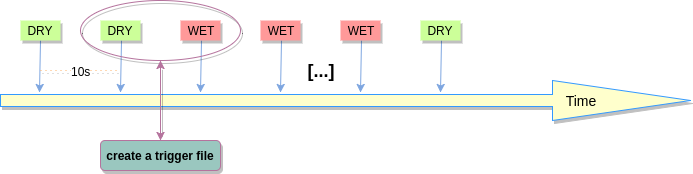
\includegraphics[width=0.9\textwidth]{includes/kom/graphics/onNotification}
  \caption{Übertragung vom Sensor zum Eval System}
  \label{fig:ble_com_pr}
\end{figure}

\paragraph{Die aktuelle Lösung} basiert daher auf dem Indication Prinzip. Nachdem der Raspi die BLE Verbindung aufgebaut hat, empängt er, wie in \ref{fig:ble_com_pr} abgebildet, die Nachrichten vom Sensor und verarbeitet diese weiter. Der Sensor sendet alle 10 Sekunden den aktuellen Status (DRY oder WET) zum Evaluation System. Somit kann auf eine Confirmation verzichtet werden, da der Raspi für die Weiterverarbeitung verantwortlich ist. Dabei muss auch nur an einer Stelle überprüft werden ob Fehler vorliegen. Ein weiterer Vorteil dieser Methode ist die schnelle Erfassung von Verbindungsfehlern während der Entwicklung.

\paragraph{Verbesserungen:} Diese Lösung hat sich stark nach der letzten Leitfrage, der einfachen Realisierung, ausgerichtet. Dennoch sind dabei viele Aspekte diskutiert worden, die eine Verbesserung in einer nächsten Version darstellen würden. Eine wesentliche Verbesserung bezüglich der Energie Bilianz des Sensors wäre nur noch das senden von Zustandsänderungen, da somit wesentlich seltener eine übertragung stattfinden würde. Des weiteren stellt die Nutzung von BLE spezifischen Funktionen, wie das abonieren von Services und die Überprüfung von Verbindungsverlusten die Möglichkeit eines einfacheren Übertragungsprotokoll dar, da somit einige Fehlerursachen bereits von dieser Schicht abstrahiert werden.

\subsubsection{Einrichtung Sensorseite}
Im aktuellen Prototyp kommt ein HM10-BLE-Modul zum einsatz. Über eine Serielle Schnittstelle kann das Modul konfiguriert und genutzt werden. Dies bietet einige Vorteile. Das Modul kommt in der Regel als Slave vorkonfiguriert und kann als solches direkt verwendet werden. Dabei werden alle Nachrichten die man an die Serielle Schnittstelle sendet auf den BLE Service mit der ID "FFEE"\todo{ überprüfen)} gemapped und über diese versendet. In der Gegenrichtung werden äquivalent alle empfangenen Nachrichten über die Serielle Schnittstelle ausgegeben. Dies ermöglicht eine einfache Nutzung der Bluetooth Low Energy Technology für kleine Projekte, da man sich nicht tiefgreifend mit dem Protokoll auseinander setzen muss. Dabei wird aber auch der Nachteil sichtbar. So ist es nicht Möglich eigene BLE Services zu definieren. Dies ist jedoch für unseren Anwendungsbereich nicht weiter von bedeutung. 

Die Konfiguration des HM10 Moduls erfolgt über sogenannte AT-Befehlen \footnote{Ursprünglich zur Kommunikation mit Modems entwickelter Befehlssatz}, welche ursprünglich zur Konfiguration von Modems entwickelt wurde. Eine Liste mit verfügbaren Kommandos ist unter \url{http://blog.blecentral.com/2015/05/05/hm-10-peripheral/} zu finden. Beim Kauf eines solchen Moduls sollte man allerdings darauf zu achten, dass man kein Plagiat bekommt, da diese in ihrer Funktionalität oftmals eingeschränkt sind. Eine Möglichkeit herauszufinden, ob man ein solches bekommen hat bietet ein Projekt von \textit{ayavilevich} welches unter \href{https://github.com/ayavilevich/arduino-ble-ident-n-set}{Github} zu finden ist.

\paragraph{Impementierung}
Um die Bedienung für das Sensorteam so einfach wie möglich zu gestallten, wurde eine C Bibliothek entwickelt, welche die Kommunikation mit dem Modul regelt. Diese stellt zwei Funktionen wie im Listing \ref{lst:bleSerial_methods} angezeigt zu Verfügung. Dabei wird die send() Methode, durch einen Interrupt Timer, zyklisch alle 10 Sekunden wie im abschnitt \ref{subsubsec:unser_protokoll} beschrieben aufgerufen. Detektiert der Sensor eine nasse Windel muss nur der Status, mittels der Funktion setState() auf "WET" umgeschaltet werden.

\begin{lstlisting}[language=C, caption=send und setState Methoden aus der BleSerial bibliothek, label=lst:bleSerial_methods ]
void BleSerial::setState(enum NapState state){
	this->mNapState = state;
};

void BleSerial::send(){
	send(mNapState);
};
\end{lstlisting}

Der komplette Code ist auf \href{https://github.com/jomaway/poop-face-detection_sensor/tree/master/arduino/libraries/BleSerial}{Github}  zu finden. \\

Wird eine Platine für den Sensor entwickelt, besteht die Möglichkeit, weiterhin ein HM10-Modul an den Mikrocontroller anzuschließen oder einen Chip mit integriertem BLE zu verwenden und dort den gleichen Service zu implementieren. In beiden Fällen muss an der Implementierung vom Evaluation System, welche im Kapitel \ref{subsubsec:ble_raspi} beschrieben wird, nichts geändert werden.

\subsubsection{Einrichtung Raspberry Pi}
\label{subsubsec:ble_raspi}
Wie weiter oben bereits erwähnt, besitzt der Raspberry Pi in der Version 3 bereits einen BLE Chip. Dadurch wird keine weiter Hardware benötigt. Auf dem Raspi läuft das Linux Betriebssystem Raspbian, welches den Bluetooth Stack bluez mitbringt. Da die Implementierung der GATT Profile auf dem Evaluation System einige Probleme mit sich bringt, wird im nächsten Abschnitt zunächst auf diese eingegangen.

\paragraph{Probleme}. \\ 
Ein wesentlicher Punkt ist die Verbreitung von Bluetooth Low Energy im allgemeinen. Während BLE bereits in vielen Projekten im Sensor-, Embedded- und Mobilbereich eingesetzt wird, ist der Einsatz auf einem klassischen Betriebssystem weniger von Bedeutung. Dadurch sind kaum brauchbare Dokumentationen und Tutorials zu diesem Thema zu finden. Zwar liefert der BLE Stack bluez seit einiger Zeit eine Implementierung für BLE Anwendungen mit, jedoch ist hier wie bei vielen Open Source Projekten, der Quellcode die einzige Dokumentation. Dadurch ist die Hürde für Einsteiger sehr hoch. Ein im Rahmen dieses Projekt entstandenes Papers "Bluetooth Low Energy Programming on Linux", welches im Anhang \ref{sec:paper_ble} beiliegt, beschreibt den Einstieg in die BLE Programmierung unter Linux. Daher wird hier nicht näher darauf eingegangen. 

\paragraph{Implementierung}. \\

Da die Videoverarbeitung und der Rest unserer Software in Python realisiert sind, setzten wir hier ebenfalls auf eine Pythonlib . Während der Test verschiedener Bibliotheken \footnote{\todo{ein paar aufzählen}} war Gattlib die einzigste, mit der sich unser Übertragungsprotokoll, wie in Kapitel \ref{subsubsec:unser_protokoll} beschrieben, problemlos implementieren lies. Listing \ref{lst:requester} zeigt einen Ausschnitt 

\begin{lstlisting}[language=Python, caption=Requester Class zur Verarbeitung der einkommenden Daten, label=lst:requester]
class Requester(GATTRequester):
    def __init__(self, wakeup, *args):
        GATTRequester.__init__(self, *args)
        self.wakeup = wakeup
        self.nap_state = "D"

    def on_notification(self, handle, data):
        data = re.sub('[^\w]', '', data)
        #ser_data = serialize_msg(data)
        print("[C] - notification on handle: {}\n".format(data))
        if(data[0] == 'W' and self.nap_state == 'D'):
            print("[C] - napkin wet")
            os.system("python3 create_trigger_file.py")
            
        self.nap_state = data[0]
        self.wakeup.set()
\end{lstlisting}

- Dateistruktur. 
- Gattlib
- Ablauf : Detektieren des Signals -> Erkennen ob neues Signal oder wieder holung des alten
  -> triggerfile erstellen.
  

\begin{figure}
  \centering
  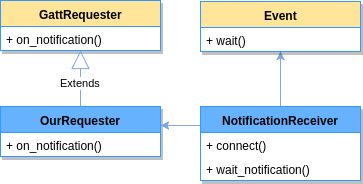
\includegraphics{includes/kom/graphics/gatt_classDiagram2}
  \caption{Klassendiagramm des Verbindungsprogramm auf dem Evaluation System}
  \label{fig:classdiagram_connection}
\end{figure}


\subparagraph{Zusammenspiel mit Aufnahemsystem}
\todo{label für triggersystem auf kapitel eval sys}


\subsection{Fazit}
\todo{Fazit verfassen}
